\documentclass[a4paper, 12pt, final, garamond]{book}
\usepackage{cours-preambule}

\raggedbottom

\makeatletter
\renewcommand{\@chapapp}{Optique -- chapitre}
\makeatother

\begin{document}
\setcounter{chapter}{1}

\chapter{Correction du TD}

\section{Fréquence, longueur d'onde et indice}
\begin{enumerate}
    \item On définit $\lambda_{r,0} = \SI{800}{nm}$ et $\lambda_{b,0} =
        \SI{400}{nm}$ les longueurs d'ondes dans le vide correspondant au
        extrémités bleue et rouge du spectre de la lumière visible.\bigbreak
        On sait que
        \begin{equation*}
            f = \frac{c}{\lambda_0}
        \end{equation*}
        On aura donc\smallbreak
        \begin{minipage}{0.45\linewidth}
            \begin{empheq}[box=\fbox]{align*}
                f_b &= \frac{c}{\lambda_{b,0}}\\
                f_r &= \frac{c}{\lambda_{r,0}}
            \end{empheq}
        \end{minipage}
        \begin{minipage}{0.45\linewidth}
            \begin{equation*}
                \text{avec}\quad
                \left\{
                    \begin{array}{rcl}
                        c & = & \SI{3.00e8}{m.s^{-1}}\\
                        \lambda_{b,0} & = & \SI{400}{nm} = \SI{4.00e-7}{m}\\
                        \lambda_{r,0} & = & \SI{800}{nm} = \SI{8.00e-7}{m}
                    \end{array}
                \right.
            \end{equation*}
        \end{minipage}\smallbreak
        L'application numérique donne
        \begin{empheq}[box=\fbox]{align*}
            f_b &= \SI{7.50e14}{Hz} = \SI{750}{THz}\\
            f_r &= \SI{3.80e14}{Hz} = \SI{380}{THz}
        \end{empheq}
    \item Dans un milieu TLHI, la longueur d'onde change de valeur selon
        \begin{equation*}
            \lambda = \frac{\lambda_0}{n}
        \end{equation*}
        Ainsi,
        \begin{enumerate}
            \item dans l'eau d'indice $n_1 = \num{1.33}$,
                \begin{empheq}[box=\fbox]{align*}
                    \lambda_{b,\rm eau} &= \SI{300}{nm} \\
                    \lambda_{r,\rm eau} &= \SI{602}{nm}
                \end{empheq}
            \item dans un verre d'indice $n_2 = \num{1.5}$,
                \begin{empheq}[box=\fbox]{align*}
                    \lambda_{b,\rm eau} &= \SI{267}{nm} \\
                    \lambda_{r,\rm eau} &= \SI{533}{nm}
                \end{empheq}
        \end{enumerate}
        Leur couleur ne change cependant pas puisque \textbf{la couleur d'une
        lumière est définie par sa fréquence/longueur d'onde dans le vide}.
    \item Dans un milieu TLHI, la vitesse de la lumière se calcule avec
        \begin{equation*}
            v = \frac{c}{n}
        \end{equation*}
        Avec $n = \num{1.5}$, on a donc
        \begin{empheq}[box=\fbox]{equation*}
            v = \SI{2.00e8}{m.s^{-1}}
        \end{empheq}
\end{enumerate}

\newpage

\section{Détermination directe de l'indice d'un liquide}
Cet exercice est d'une simplicité absolue. Et pourtant...
\begin{tcbraster}[raster columns=5, raster equal height=rows]
    \begin{NCdefi}[raster multicolumn=3, sidebyside, righthand width=4cm]{Données}
        \begin{enumerate}
            \item Rayon incident sur un dioptre entre air et milieu d'indice $n$ :
                angle {\huge avec le dioptre} de \ang{56;;} ;
            \item Différence d'angle entre rayon incident et réfléchi (« déviation
                ») de \ang{13.5;;}.
        \end{enumerate}
        \tcblower
        \begin{center}
            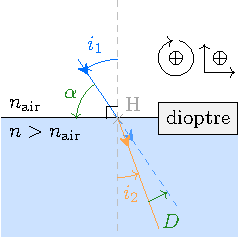
\includegraphics{dioptre_alpha-horiz.pdf}
        \end{center}
    \end{NCdefi}    
    \begin{tcolorbox}[blankest, raster multicolumn=2, space to=\myspace]
        \begin{tcbraster}[raster columns=1]
            \begin{NCprop}[add to natural height=\myspace]{Résultat attendu}
                Indice du liquide.
            \end{NCprop}
            \begin{NCrapp}{Outils du cours}
                Loi de Snell-Descartes :
                \[ n_1\sin i_1 = n_2 \sin i_2 \]
                avec $n_1$ l'indice du milieu d'incidence, $n_2$ celui du milieu
                de réfraction, $i_1$ l'angle d'incidence et $i_2$ l'angle de
                réfraction.
            \end{NCrapp}
        \end{tcbraster}
    \end{tcolorbox}
\end{tcbraster}

\begin{NCexem}{Application}
    Un bon schéma fait attentivement est \textbf{nécessaire} ici. En effet,
    les angles donnés ne sont pas ceux qu'on utilise dans la relation de
    Snell-Descartes. \bigbreak
    
    En appelant $\alpha$ l'angle entre le rayon et le dioptre, on a
    \[ \alpha + i_1 = \ang{90;;}\]
    donc \fbox{$i_1 = \ang{34;;}$}. Et en appelant $D$ la déviation entre
    les deux rayons, on a
    \[ i_1 = i_2 + D\]
    soit \fbox{$i_2 = \ang{20.5;;}$}. On en déduit donc
    \[\boxed{n = \frac{\sin i_1}{\sin i_2}} \quad \text{avec} \quad
        \left\{
            \begin{array}{rcl}
                i_1 & = & \ang{34;;}\\
                i_2 & = & \ang{20.5;;}
            \end{array}
    \right. \quad \text{soit} \quad \boxed{n = 1.6}
    \]
\end{NCexem}

\section{Détecteur de pluie sur un pare-brise}
On modélise un pare-brise par une lame de verre à faces parallèles, d'épaisseur
$e = \SI{5.00}{mm}$, d'indice $n_v = \num{1.5}$. Un fin pinceau lumineux issu d'un
émetteur situé en $E$ arrive de l'intérieur du verre sur le dioptre verre
$\rightarrow$ air en $I$ avec un angle d'incidence $i = \ang{60.;;}$.
\begin{enumerate}
    \item Pour savoir si le pinceau lumineux revient intégralement, il faut
        savoir s'il y a réflexion totale à l'interface verre$\rightarrow$air.
        Pour cela, on utilise la formule de l'angle limite de réfraction
        \begin{equation*}
            i_{\rm lim} = \arcsin \left( \frac{n_2}{n_1} \right)
        \end{equation*}
        Ici, on a
        \[\boxed{i_{\rm lim, v\rightarrow a} =
            \arcsin \left( \frac{n_{\rm air}}{n_{\rm verre}} \right)}
        \quad\text{avec}\quad
        \left\{
            \begin{array}{rcl}
                n_{\rm air} & = & \num{1.00}\\
                n_{\rm verre} & = & \num{1.5}
            \end{array}
        \right.
        \]
        L'application numérique donne
        \begin{empheq}[box=\fbox]{equation*}
            i_{\rm lim, v\rightarrow a} = \ang{41.8;;}
        \end{empheq}
        Comme $i = \ang{60.;;}$, $i > i_{\rm lim v\rightarrow a}$, et on a
        donc réflexion totale~: aucun rayon ne sera réfracté.\bigbreak
        Avec la figure ci-après, on a $\tan(i) = \frac{ED}{2e}$, soit
        \[\boxed{ED = 2e\tan(i)}
        \quad\text{avec}\quad
        \left\{
            \begin{array}{rcl}
                e & = & \SI{5.00}{mm}\\
                i & = & \ang{60.;;}
            \end{array}
        \right.\]
        L'application numérique donne
        \begin{empheq}[box=\fbox]{equation*}
            ED = \SI{1.7}{cm}
        \end{empheq}
    \item Dans le cas où une fine couche d'eau recouvre le verre, on doit
        calculer le nouvel angle limite de réfraction pour l'interface
        verre$\rightarrow$eau. Comme précédemment, on utilise la formule et on
        trouve
        \begin{empheq}[box=\fbox]{equation}
            i_{\rm lim, v\rightarrow e} = \ang{62.5;;}
        \end{empheq}
        Cette fois, l'angle d'incidence $i < i_{\rm lim, v\rightarrow e}$. On va
        donc avoir réfraction. On détermine l'angle de réfraction $i_2$ avec la
        loi de Snell-Descartes pour la réfraction~: $n_2\sin(i_2) =
        n_1\sin(i_1)$. Dans notre cas, $n_2 = n_{\rm eau}$, $n_1 = n_{\rm
        verre}$ et $i_1 = i$~; on aura donc
        \[\boxed{i_2 = \arcsin \left(
            \frac{n_{\rm verre}\sin(i)}{n_{\rm eau}}
        \right)}
        \quad\text{avec}\quad
        \left\{
            \begin{array}{rcl}
                n_{\rm verre} & = & \num{1.5}\\
                i & = & \ang{60.;;}\\
                n_{\rm eau} & = & \num{1.33}
            \end{array}
        \right.\]
        D'où
        \begin{empheq}[box=\fbox]{equation*}
            i_2 = \ang{77.6;;}
        \end{empheq}
        Ce rayon réfracté (en vert sur la figure) va ensuite rencontrer le
        dioptre eau$\rightarrow$air en $J$, pour lequel l'angle limite de
        réfraction est
        \begin{empheq}[box=\fbox]{equation*}
            i_{\rm lim, e\rightarrow a} = \ang{48.8;;}
        \end{empheq}
        Comme $i_2 > i_{\rm lim, e\rightarrow a}$, on a une nouvelle réflexion
        totale avec $r=-i_2$, ramenant le pinceau vers le dioptre
        eau$\rightarrow$verre en un point $K$. Dans cette situation comme la
        valeur absolue de $r$ est la même que celle de $i_2$, le principe
        du retour inverse de la lumière nous permet de déterminer directement
        que l'angle de réfraction de l'eau vers le verre $i_3$ a la même valeur
        absolue que l'angle d'incidence du verre vers l'eau $i_1$.\bigbreak

        Avec le schéma ci-après, on peut déterminer que $DL = IK$ (l'abscisse
        supplémentaire du trajet dans l'eau) et utiliser la trigonométrie pour
        trouver
        \[\boxed{IK = 2e'\tan(i_2)}
        \quad\text{avec}\quad
        \left\{
            \begin{array}{rcl}
                e' & = & \SI{1.00}{mm}\\
                i_2 & = & \ang{77.6;;}
            \end{array}
        \right.\]
        soit
        \begin{empheq}[box=\fbox]{equation*}
            DL = \SI{0.9}{cm}
        \end{empheq}
        Ainsi, le rayon ne tombe plus sur le détecteur mais à côté~; un système
        de commande relié au détecteur peut alors déclencher les essuie-glaces.
\end{enumerate}
\begin{figure}[h]
    \centering
    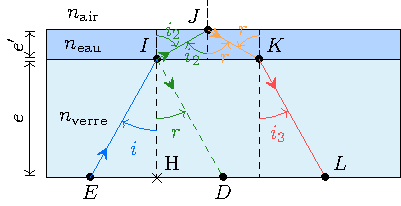
\includegraphics[width=\linewidth]{pluie.pdf}
    \label{fig:pluie_plain}
\end{figure}

\section{Rayon lumineux à travers une vitre}

\begin{tcbraster}[raster columns=11, raster equal height=rows]
    \begin{tcolorbox}[blankest, raster multicolumn=5, space to=\myspace]
        \begin{tcbraster}[raster columns=1]
            \begin{NCdefi}[raster multicolumn=1]{Schéma}
                \begin{center}
                    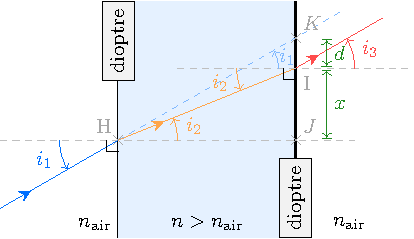
\includegraphics{vitre}
                \end{center}
            \end{NCdefi}
            \begin{NCrapp}[add to natural height=\myspace]{Outils}
                Loi de Snell-Descartes :
                \[n_1\sin i_1 = n_2\sin i_2\]
            \end{NCrapp}
        \end{tcbraster}
    \end{tcolorbox}
    \begin{tcolorbox}[blankest, raster multicolumn=6, space to=\myspace]
        \begin{tcbraster}[raster columns=1]
            \begin{NCprop}[raster multicolumn=6]{Résultat attendu}
                Le rayon passe deux dioptres de l'air au verre, puis
                du verre à l'air. On utilise Snell-Descartes pour déterminer la
                direction du rayon émergent et la comparer à celle du rayon
                incident.
            \end{NCprop}
            \begin{NCexem}[sidebyside, righthand width=1.5cm,
                add to natural height=\myspace]{Application}
                \begin{itemize}[leftmargin=40pt]
                    \item[\textbf{En H}] : $\sin i_1 = n\sin i_2$\smallbreak
                        \hspace{-40pt}$\Leftrightarrow
                        i_2 = \arcsin(\sin(i_1)/n) = \ang{28;;}$;
                    \item[\textbf{Dedans}] : $i_2$ aux deux dioptres ;
                    \item[\textbf{En I}] : $\sin i_3 = n\sin i_2$ ;
                    \item[\textbf{D'où}] :
                        $\cancel{n_1}\sin i_3 = \cancel{n_1}\sin i_1$
                \end{itemize}
                \tcblower
                Finalement,
                \[\boxed{i_3 = i_1}\]
                (retour inverse)
            \end{NCexem}
        \end{tcbraster}
    \end{tcolorbox}
\end{tcbraster}
\begin{enumerate}[start=3]
    \item Comme les dioptres sont parallèles, leurs normales le sont aussi.
        Ainsi, les rayons émergent et incident sont parallèles.
    \item $\DS\tan(i_2) = \frac{IJ}{HJ} = \frac{x}{a}$ et $\DS\tan(i_1) =
        \frac{x+d}{a}$, d'où $\DS\frac{d}{a} = \tan(i_1) - \frac{x}{a} = \tan(i_1)
        - \tan(i_2)$, soit
        \[\boxed{d = a(\tan(i_1) - \tan(i_2))}
        \quad\text{avec}\quad
        \left\{
            \begin{array}{rcl}
                a & = & \SI{5.0}{mm}\\
                i_1 & = & \ang{45;;}\\
                i_2 & = & \ang{28;;}
            \end{array}
        \right.\]
        C'est-à-dire
        \begin{empheq}[box=\fbox]{equation*}
            d = \SI{2.3}{mm}
        \end{empheq}
\end{enumerate}

\section{Fibre optique à saut d'indice}

\begin{figure}[h]
    \centering
    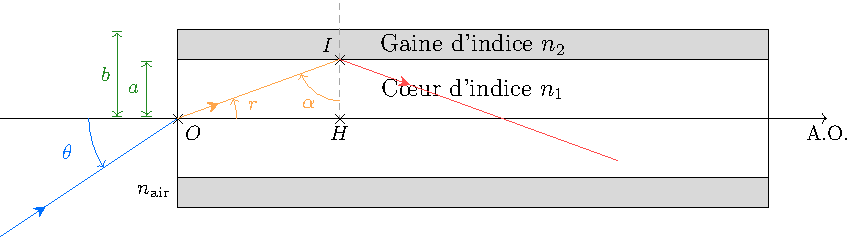
\includegraphics[width=.8\linewidth]{fibre.pdf}
    \captionsetup{justification=centering}
    \caption{Schéma d'une fibre optique à saut d'indice.}
    \label{fig:fibre}
\end{figure}

\begin{multicols}{2}
    \begin{itemize}
        \item[En O] : $\sin(\theta) = n_1\sin(r) \Leftrightarrow \fbox{$\DS\sin(r) =
            \frac{\sin(\theta)}{n_1}$}$~;
        \item[OIH] : $\alpha = \DS \frac{\pi}{2} - r$~;
        \item[En I] : On veut $\sin(\alpha) \geq \DS\frac{n_2}{n_1}$~;
        \item[$\alpha\rightarrow r$] : $\sin(\alpha) = \sin(\pi/2 -r) =
            \cos(r)$\\
            \fbox{$\DS\sin(\alpha) \geq \frac{n_2}{n_1} \Leftrightarrow \cos(r) \geq
            \frac{n_2}{n_1}$}
    \end{itemize}
    \columnbreak
    \begin{itemize}[leftmargin=100pt]
        \item[$\cos(r)\rightarrow\sin(r)$] : $\cos^2(r) = 1-\sin^2(r)$~;
        \item[$r\rightarrow\theta$] : $\sin^2(r) = \DS
            \frac{\sin^2(\theta)}{n_1{}^2}$~;
        \item[Combinaison] : $n_1{}^2 - \sin^2(\theta) \geq n_2{}^2$~;
        \item[Conclusion] : \fbox{$\theta \leq \arcsin \left( \sqrt{n_1{}^2 -
            n_2{}^2} \right)$}
    \end{itemize}
\end{multicols}

\section{Mirages}

\begin{wrapfigure}[13]{R}{.5\linewidth}
    \vspace*{20pt}
    \centering
    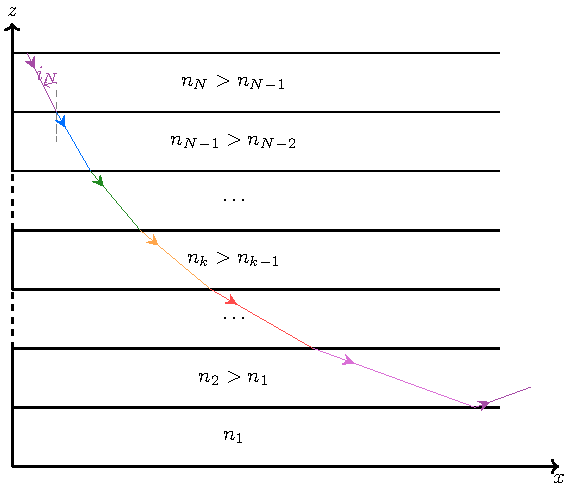
\includegraphics[width=\linewidth]{mirage}
    \captionsetup{justification=centering}
    \caption{Rayons d'un mirage chaud}
    \label{fig:mirage}
\end{wrapfigure}
~
\begin{enumerate}
    \item 
    \begin{enumerate}
        \item À chaque interface, $n_k\sin(i_k) = n_{k-1}\sin(i_{k-1})$~;
            notamment, avec $k=2$, on a $n_2\sin(i_2) = n_1\sin(i_1)$. Ainsi,
            tous les $n_k\sin(i_k)$ sont égaux.
        \item Voir figure ci-après.\smallbreak
            À chaque «~dioptre~», on a $\sin(i_{\rm lim, k}) =
            \frac{n_{k-1}}{n_k}$. Sa valeur maximale est à $k=2$~: $\sin(i_{\rm
            lim,2}) = \frac{n_1}{n_2}$. Comme $n_k\sin(i_k)$ est constant et que
            $n_k$ diminue, on sait que $i_k$ augmente~: ainsi, si l'angle
            d'incidence $i_N$ est suffisamment grand, il y aura un $i_k$
            supérieur à $i_{\rm lim,2}$ et donc réflexion totale.
        \item Voir figure.
        \item Alors qu'on devrait voir le sable, les rayons venant du haut des
            collines sont déviés vers le haut~: on a l'impression de voir à
            travers la dune.
    \end{enumerate}
\end{enumerate}

\begin{enumerate}[start=2]
    \item Cette fois ce sont les rayons dirigés vers le haut d'un objet lointain
        qui sont déviés vers le bas~: on a l'impression de voir des objets
        au-dessus du niveau de la mer. Schéma non fourni.
\end{enumerate}

\section{Réfractomètre de Pulrich}
\begin{wrapfigure}[6]{R}{.3\linewidth}
    \vspace*{20pt}
    \centering
    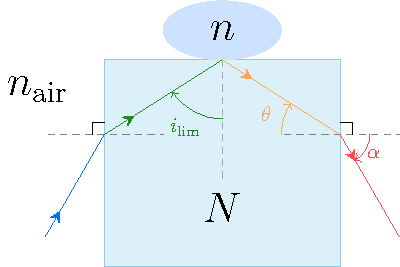
\includegraphics[width=\linewidth]{pulrich}
    \label{fig:pulrich_plain}
\end{wrapfigure}
~
\begin{enumerate}
    \item $\DS \sin(i_{\rm lim, N\rightarrow n}) = \frac{n}{N}$ d'une part. D'autre
        part, $N\sin(\theta) = \sin\alpha$, mais on a aussi $\theta = \pi/2 -
        i_{\rm lim}$~: on a donc $\sin\theta = \cos i_{\rm lim} = \DS \sqrt{1-
        \left(\frac{n}{N}\right)^2}$. Ainsi, $\DS\sin^2\alpha = N^2 \left( 1 -
    \frac{n^2}{N^2} \right)$~; autrement dit,
    \begin{equation*}
        \boxed{n = \sqrt{N^2 - \sin^2\alpha}}
        \quad\text{avec}\quad
        \left\{
            \begin{array}{rcl}
                N & = & \num{1.622}\\
                \alpha & = & \ang{60;;}
            \end{array}
        \right.
    \end{equation*}
    \item Application numérique~:
        \[\boxed{n = \num{1.376}}\]
\end{enumerate}

\section{Incidence de Brewster}

Les rayons réfléchis et réfractés sont perpendiculaires si $r+i =
\frac{\pi}{2} \Leftrightarrow r = \frac{\pi}{2} -i$. En venant de l'air, on a
$\sin i = n\sin r$, soit $\sin i = n\cos i$~; autrement dit
\begin{equation*}
    \boxed{\tan i = n}
\end{equation*}

\section{Réfraction et dispersion}

La lumière blanche est constituée d'une superposition de longueurs d'onde dans
le vide entre \SIrange{400}{800}{nm}. Quand ce faisceau arrive sur
le dioptre et passe dans le milieu, l'indice de réfraction, qu'on utilise dans
la relation de Snell-Descartes, change selon la longueur d'onde dans le vide.
Pour une même valeur de $i$ incident on aura donc deux valeurs extrêmes de $r$
réfracté, que l'on nomme $r_b$ et $r_r$ pour «~bleu~» et «~rouge~», selon~:

\begin{minipage}{0.49\linewidth}
    \begin{empheq}[box=\fbox]{align*}
        n_{\rm air}\sin(i) &= n_b\sin(r_b)\\
        n_{\rm air}\sin(i) &= n_r\sin(r_r)
    \end{empheq}
\end{minipage}
$\Longleftrightarrow$
\begin{minipage}{0.49\linewidth}
    \begin{empheq}[box=\fbox]{align*}
        r_b &= \arcsin \left( \frac{n_{\rm air}\sin(i)}{n_b} \right)\\
        r_r &= \arcsin \left( \frac{n_{\rm air}\sin(i)}{n_r} \right)
    \end{empheq}
\end{minipage}

Comme $\lambda_{0,b} < \lambda_{0,r}$, $\underbrace{n(\lambda_{0,b})}_{n_b} >
\underbrace{n(\lambda_{0,r})}_{n_r}$ et
forcément $r_b < r_r$. On calcule~:

\begin{minipage}{0.49\linewidth}
    \begin{empheq}[box=\fbox]{align*}
        n_b &= \num{1.53}\\
        n_r &= \num{1.51}
    \end{empheq}
\end{minipage}
$\Longleftrightarrow$
\begin{minipage}{0.49\linewidth}
    \begin{empheq}[box=\fbox]{align*}
        r_b &= \ang{24.8;;}\\
        r_r &= \ang{25.2;;}
    \end{empheq}
\end{minipage}

L'écart angulaire est donc
\[\boxed{\theta = r_r - r_b = \ang{0.35;;}}\]

\begin{figure}[h]
    \centering
    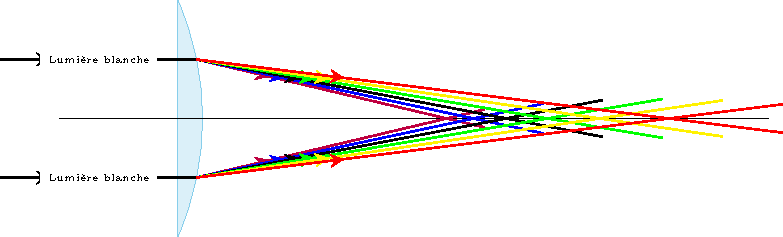
\includegraphics[width=.61\linewidth]{abbe_chroma.pdf}
    \captionsetup{justification=centering}
    \caption{Exemple (exagéré) de dispersion (aberration chromatique).}
    \label{fig:aberr}
\end{figure}

\end{document}
